\documentclass[crop, tikz]{standalone}

\usepackage[utf8]{inputenc}
% 'crop' is the default for v1.0, before it was 'preview'
%\usetikzlibrary{...}% tikz package already loaded by 'tikz' option

\usetikzlibrary{arrows}
\usetikzlibrary{decorations.markings}
\usetikzlibrary{patterns}
\usetikzlibrary{calc}

%hexagon drawing variables
\def\ly{0.866025} %sin(pi/3) = sqrt(3)/2
\def\lx{0.5} %cos(pi/3) = 0.5
\def\hexSize{5} %size of the hexagon that'll be the extent of the fibre cross section
\def\coreSize{0.2} %size of hollow cores
\def\coreSep{0.5} %separation between core CENTRES HORIZONTALLY
\def\coreSepHeight{0.4464} %separation between core CENTRES VERTICALLY

\newcommand{\hexagon}[4]{
\begin{scope}[shift={#2}]
	\draw[#3, fill=#4] (-#1*\lx, #1*\ly) -- (#1*\lx, #1*\ly) -- (#1,0) -- (#1*\lx, -#1*\ly) -- (-#1*\lx, -#1*\ly) -- (-#1,0) -- cycle;
\end{scope}
} %\hexagon{centre-to-corner-length}{shift (x,y)}{line spec}{fill colour} [none is allowed for fillcolour]

\begin{document}
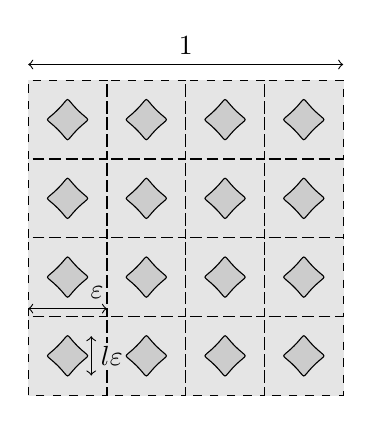
\begin{tikzpicture}[]
	
	% boundary of \ddom_h
	\filldraw[black!10!white] (0,0) rectangle (4,4);

	\foreach \x in {0,1,...,3} {
		\foreach \y in {0,1,...,3} {
			\begin{scope}[shift={(\x,\y)}, scale=0.25]
				\filldraw[black!20!white, draw=black] plot [smooth cycle, tension=2.5] coordinates {(1.5,1.5) (2.5,1.5) (2.5,2.5) (1.5,2.5)};
				\draw[dashed] (0,0) rectangle (4,4);
			\end{scope}
		}
	}
	
	% length scale labels
	% domain size
	\draw[<->] (0,4.2) -- (4,4.2); \node[anchor=south] at (2,4.2) {$1$};
	% period cell size
	\draw[<->] (0,1.1) -- (1,1.1); \node[anchor=south] at (0.875,1.1) {$\varepsilon$};
	% inclusion size (also cut out a small box to make text easier to read
	\filldraw[black!10!white] (0.95,0.35) rectangle (1.05,0.65);
	\draw[<->] (0.8,0.25) -- (0.8,0.75); \node[anchor=west] at (0.8,0.5) {$l\varepsilon$};

\end{tikzpicture}
\end{document}